\subsubsection{Memory Usage}

Charts on Figures \ref{fig:persistent_client_transport_memory}, \ref{fig:ephemeral_client_transport_memory}, \ref{fig:persistent_server_transport_memory}, and \ref{fig:ephemeral_server_transport_memory} represent the memory usage of clients and servers during ephemeral and persistent experiments.

\subsubsection*{Overall Memory Cost}

During persistent and ephemeral experiments, it’s possible to observe that \gls{udp} and \gls{tcp} had the lowest memory usage. However, \gls{tcp}+\gls{tls} was more than double. That can be explained by \gls{tls}’ data encryption overhead, which demands a bit more memory usage.

\subsubsection*{QUIC Unusual Ephemeral Client Memory Cost}

QUIC uses around double memory when compared to \gls{tcp}+\gls{tls} experiments. Nothing special since it’s expected to have more memory usage as a tradeoff for efficiency on unreliable networks. Nonetheless, during ephemeral experiments it had an interesting behaviour. On smaller payloads it uses a ton of memory, almost 10 times \gls{tcp}+\gls{tls}’, while only using half with larger payloads (Figure \ref{fig:ephemeral_client_transport_memory} and \ref{fig:ephemeral_server_transport_memory}).

This happens during ephemeral experimentations only because the application is constantly creating and deleting clients, therefore Go’s garbage collector is unable to quickly clean unused clients. On smaller payloads, the rate of client creation is higher because the requests end faster, in contrast to larger payloads, which require more time to complete requests, allowing Go’s garbage collector more time to do its job. This behaviour is intensified during QUIC’s experiments due to its higher cost when creating clients.

\clearpage

\begin{figure}[h!]
    \centering
    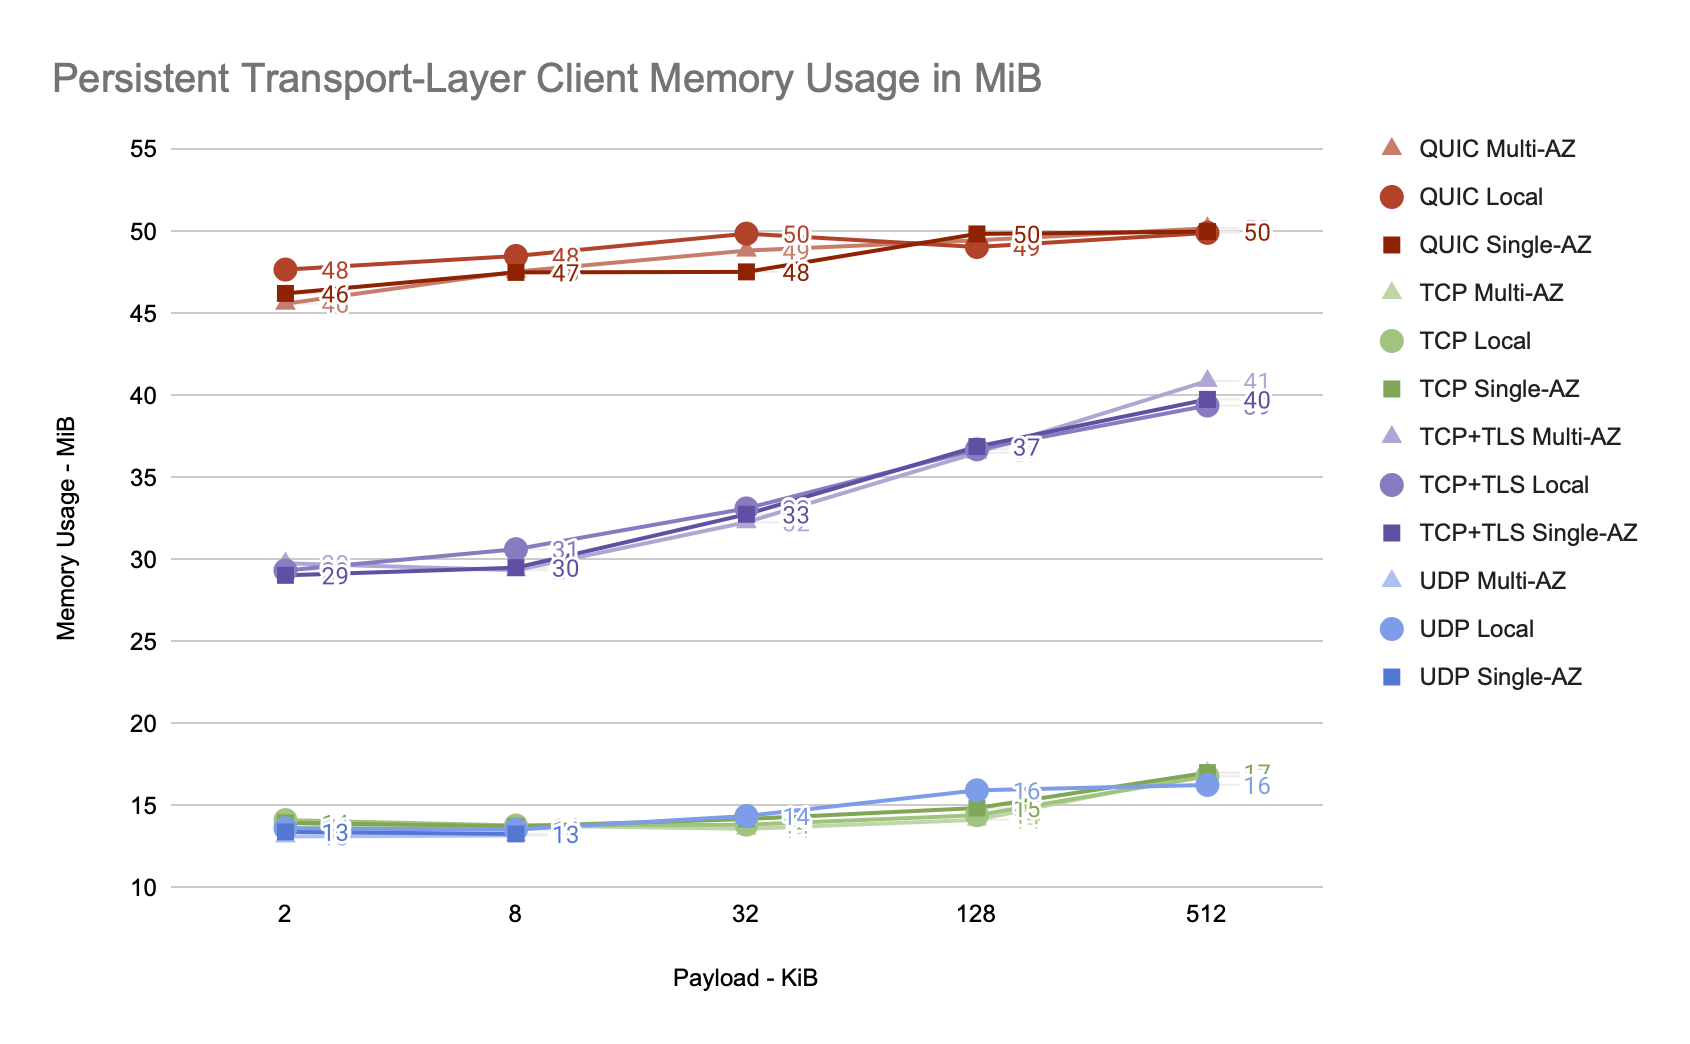
\includegraphics[width=\linewidth]{figures/charts/Persistent Transport-Layer Client Memory Usage in MiB.png}
    \caption{Persistent Transport-Layer Client Memory Usage in MiB}
    \label{fig:persistent_client_transport_memory}
\end{figure}

\begin{figure}[h!]
    \centering
    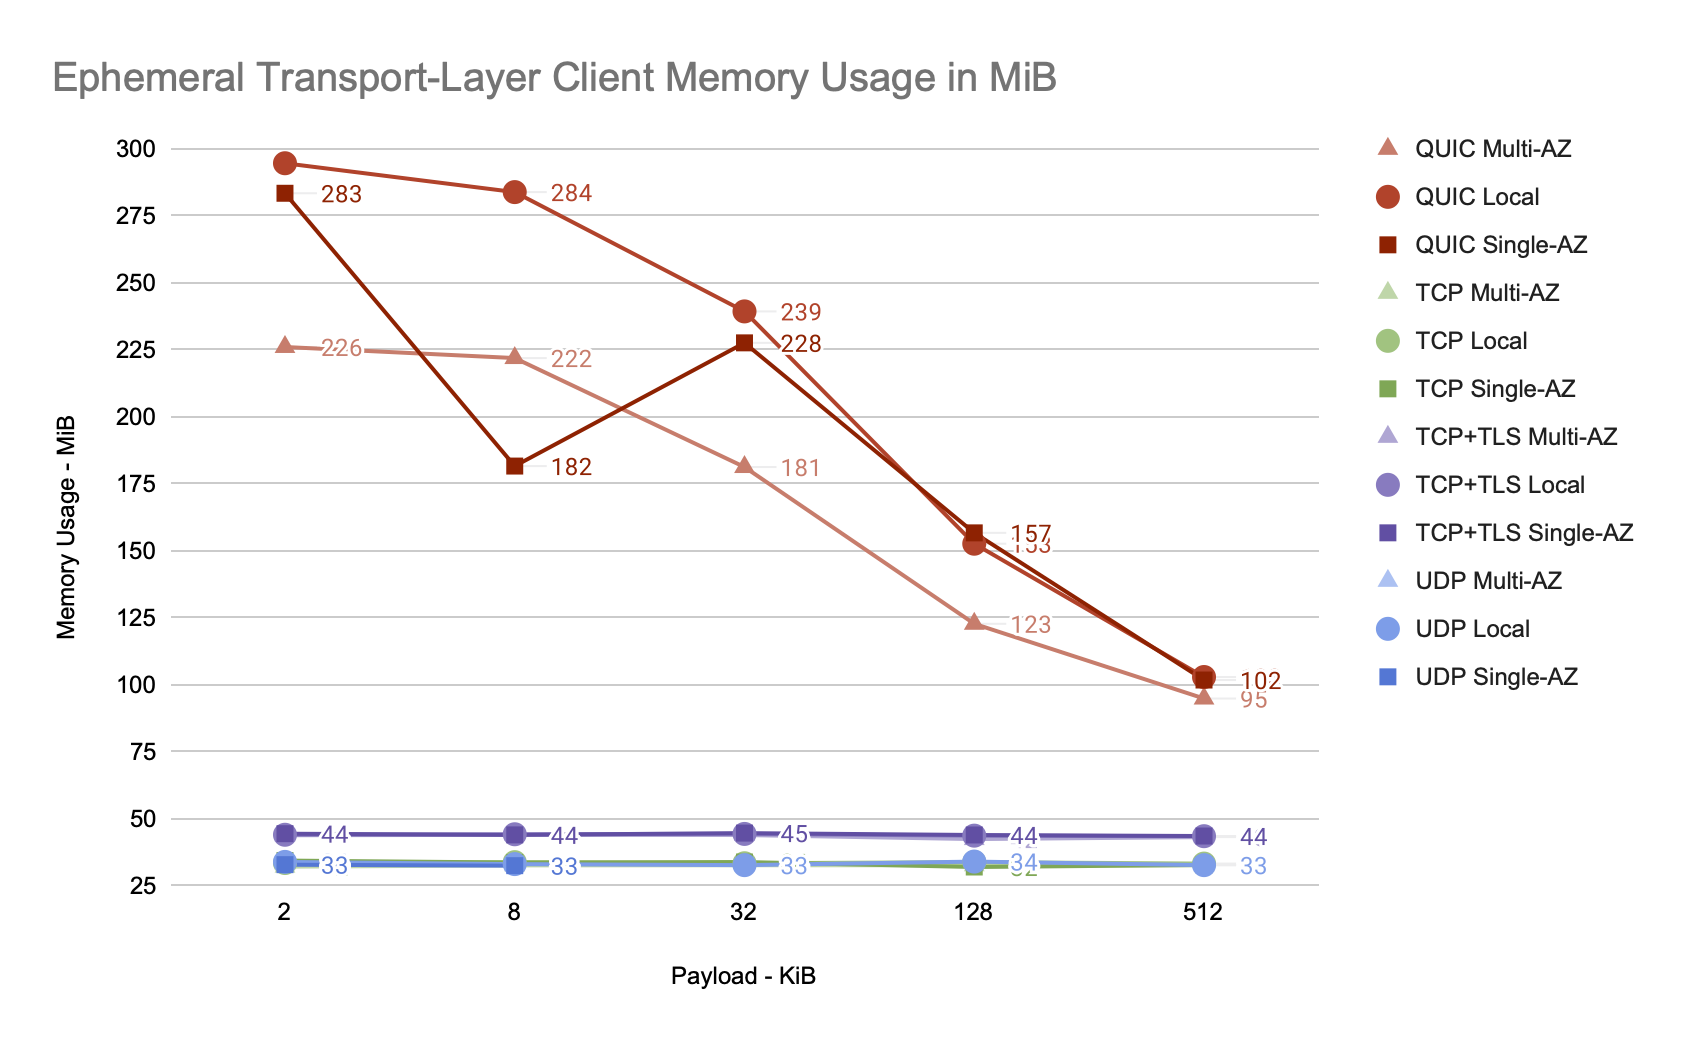
\includegraphics[width=\linewidth]{figures/charts/Ephemeral Transport-Layer Client Memory Usage in MiB.png}
    \caption{Ephemeral Transport-Layer Client Memory Usage in MiB}
    \label{fig:ephemeral_client_transport_memory}
\end{figure}

\clearpage

\begin{figure}[h!]
    \centering
    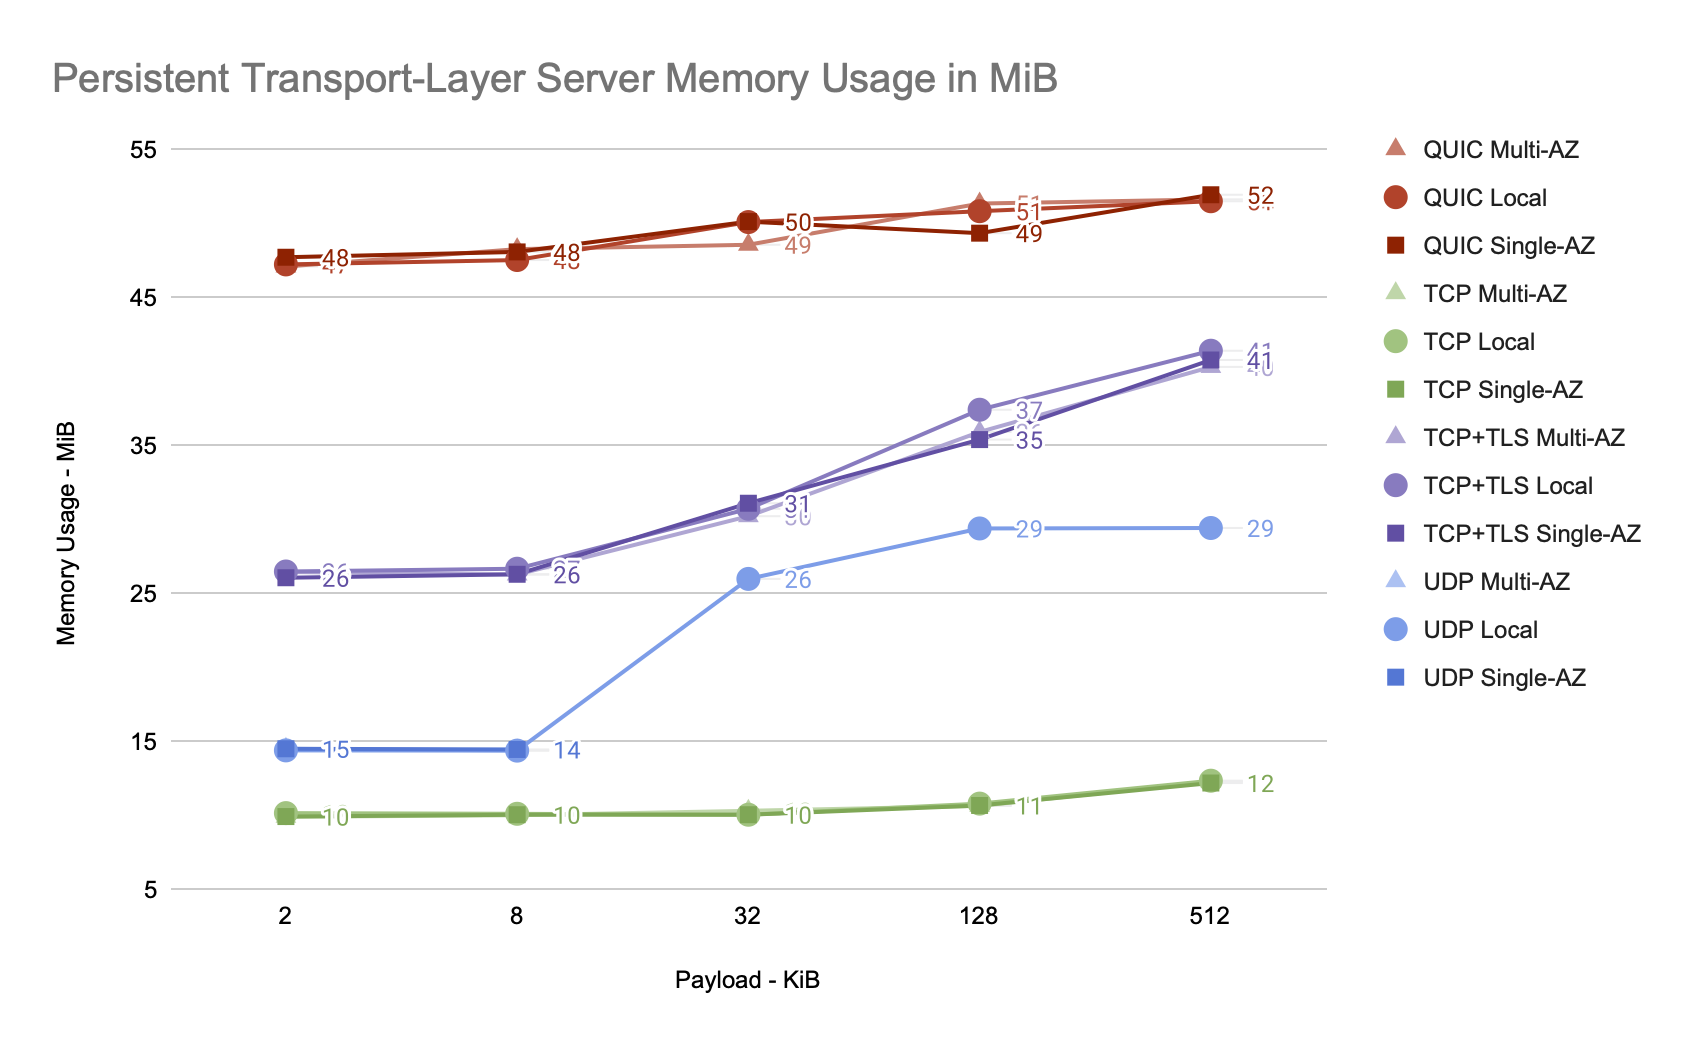
\includegraphics[width=\linewidth]{figures/charts/Persistent Transport-Layer Server Memory Usage in MiB.png}
    \caption{Persistent Transport-Layer Server Memory Usage in MiB}
    \label{fig:persistent_server_transport_memory}
\end{figure}

\begin{figure}[h!]
    \centering
    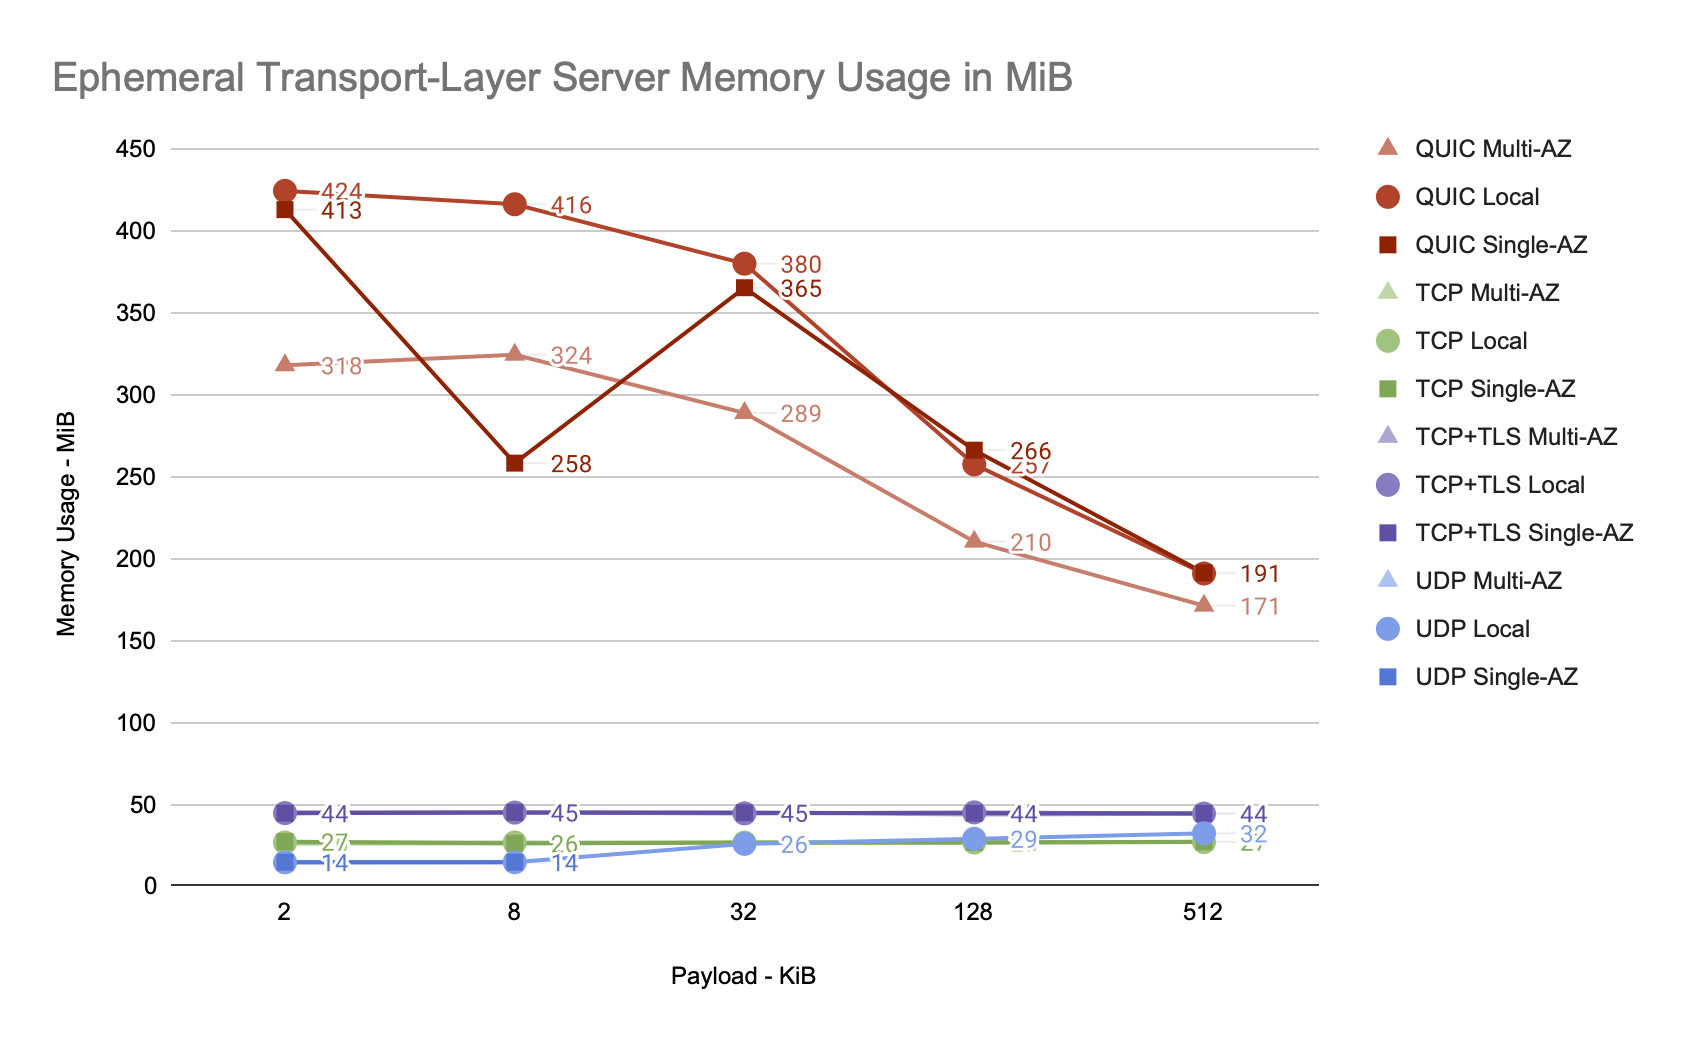
\includegraphics[width=\linewidth]{figures/charts/Ephemeral Transport-Layer Server Memory Usage in MiB.png}
    \caption{Ephemeral Transport-Layer Server Memory Usage in MiB}
    \label{fig:ephemeral_server_transport_memory}
\end{figure}

\clearpage
